% !TeX root = ../thesis.tex
%*****************************************************************************************
%*********************************** First Chapter ***************************************
%*****************************************************************************************

\newcommand{\pd}[2]{\frac{\partial #1}{\partial #2 }}
\newcommand{\td}[2]{\frac{d #1}{d #2 }}
\newcommand{\mb}[1]{\mathbf{#1}}
\newcommand{\divv}[1]{\bigtriangledown{#1}}
\newcommand{\del}{\bigtriangledown}

\label{ch:Intro}
\chapter{Introduction}  %Title of the First Chapter


%%%%%%%%%%%%%%%%%%%%%%%%%%%%%%%%%%%%%%%%%%%%%%%%%%%%%%%%%%% PAPER TEXT %%%%%%%%%%%%%%%%%%%%%%%%%%%%%%%%%%%%%%%%%%%%%%%%%%%%%%%%%%%%%%%%%%%%%%%%%%%%%%



\section{The Sun}
The Sun is an extremely complex system, consisting primarily of ionised plasma, the formation of which generated the collection of planets and asteroids we call the solar system.
As such, the study of our nearest star should be at the forefront of our research into the cosmos; any model we build to examine other stars must first accurately describe our star. 
The Sun takes its place on the Hertzsprung-Russell [\cite{Hertzsprung1909, Russell1914}] diagram as an early life main sequence star at the yellow end of the stellar spectrum.
It is a population 3 star, meaning that it has a high metallic content, a fact which aids in our observations immeasurably.

\subsection{Solar Interior}

The structure of the Sun can be divided into internal and external regions.
Internal structure has been inferred by the use of techniques such as Helio seismology, therefore we still have many questions as to the exact mechanisms dominating below the photosphere.
At the centre is the solar core, wherein fusion takes place. 
Followed by the radiative zone, tachocline and convective zone.

The tachocline has the greatest impact on the solar atmosphere, as it has also been proposed as the source for a dynamo generating the magnetic field.
The most important result of the tachocline is that at this point, the motion changes from uniform behaviour of the radiation zone to the differential rotation of the convective zone.
This differential rotation is the cause of extremely complex global magnetic field permeating the Sun.
The tachocline, as discussed in \cite{Brun2001}, is a thin layer between the radiative zone and the convection zone, of which not a great deal is known.
A particular impact of the tachocline's existence, is that the $p-mode$ oscillations used in helioseismology, interact strongly with it, as demonstrated in \cite{Chaplin2014}, to the point of filtering high order oscillations out.
There have been recent studies, such as \cite{Obridko2007} which suggest that the tacholine is responsible for several $1.3$ to $3$ year cycles in feature observed higher in the solar atmosphere, however this has not been definitively proven.

Above the tachocline, there is the onset of convection, naming this region of the solar interior.
The convective cells of heating and cooling plasma carries the magnetic field from the tachocline up to the bottom of the photosphere.
The tops of these cooling cells, hotter plasma in the centre and cooler, darker, plasma at the edges form the granulation ubiquitous in any image of the photosphere [\cite{Nordlund2009}].


\subsection{The solar atmosphere}
The photosphere is the minima of the solar temperature profile, with a temperature range starting at $6000$ K at the base, and $4700$ K at the top.
It emits light in the visible band of the electromagnetic spectrum, a fact utilised in spectrascopic imaging of the solar atmosphere.
The granulation resulting from the convective region appears as dark lines and bright 'bubbles' expanding and collapsing as hot material rises, cools and consequently falls back down into the solar interior, [\cite{Nordlund2009}].
These features tend to measure approximately $2$ Mm from one boundary to the other, which, are know as inter-granular lanes.

%\begin{figure}
%	\centering
%	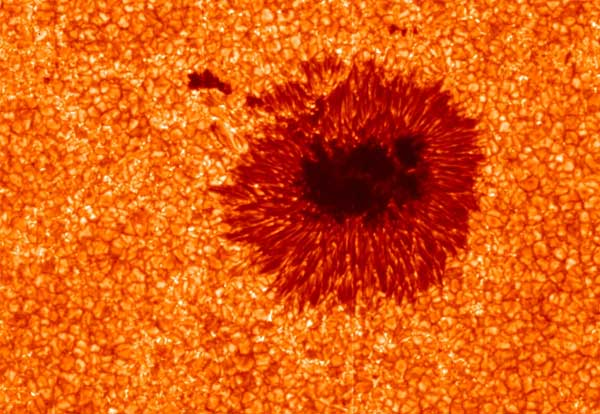
\includegraphics[width=0.75\textwidth]{Chapter1/Figs/granulation_and_sunspot}
%	\caption{An image of the photosphere featuring its most prominent structures. The sunspot is comprised of the Umbra, dark plasma at the centre, and Penumbra, the thin structures leading away from the Umbra. It is through the Umbra that the magnetic field emerges, causing a lowering of temperature, hence its dark appearance.
%	The rest of the image is dominated by granulation. See the tops of the cells as bright plasma surrounded by the darker, cooler, intergranular lanes
%		\url{https://www.aps.org/units/dfd/pressroom/papers/sun.cfm}}
%	\label{fig:granssp}
%\end{figure}

%TODO add sunspot references
The most prominent feature in the photosphere are sunspots.
These features are significantly cooler that the surrounding photosphere, with a dark centre, known as the umbra, through which open magnetic field emerges from the solar interior.
Spreading away from the umbra is the penumbra, a ring of long thin structures spreading away from the umbra.
These have been widely studied and have become known as fibrils.
The reason these are so widely studied, is that it has become clear that waves travel up these features from the solar interior.
Sunspots are normally part of an extremely complex system of magnetic field, meaning that there are usually many in one active region.
Sunspots are widely used as indicators of solar activity, the study of them has lead to the discovery of the 11 and 22 year solar cycles.
Analysis of their locations has also lead to the proposition of an active longitude, where sunspot formation is more frequent, the testing of this concept with macrospicules is the subject of 
%TODO citation for solar cycles discovery
The photosphere is the coolest point in the solar temperature profile, from this point the temperature of the solar atmosphere will continue to increase with distance from the photosphere.

The layer above the photosphere, is the chromosphere, so called, as when observed during solar eclipses, it appears colourful.
The density drops sharply from the photosphere to the order of $10^{-4}$ and is approximately $2$ Mm thick. 
Over this $2$ Mm layer the temperature rises from $4000$ K to $25,000$ K, see \emph{e.g.} \cite{Withbroe1977}.
This result is currently one of the primary focuses of the solar research community.
The chromosphere is incredibly complex in terms of its magnetic structure and the transport of heat, consequently the chromosphere plays an essential role in the formation of explosive events such as solar flares and coronal mass ejections (CMEs).

Prevalent in the chromospheric, and subsequently the coronal spectral lines, are the magnetic field lines which are rooted in the sunspots, demonstrated in \cite{Athay1976}.
These appear as large-scale loops of plasma which has been locked into the magnetic field lines, extending through this region and right into the corona, they regularly reach $10$s of Mm into the atmosphere.
Lower in the chromosphere, we find a second, smaller-scale population of loops, and are a few Mm across on average.
Small-scale chromospheric loops have been presented as a possible link between the photosphere and the chromosphere, due the their most likely formation being a small-scale flux emergence event [\cite{Ulmschneider1982}].

Particularly noticeable in the chromosphere are the footprints of the coronal holes, a review of which can be found in \cite{Cranmer2009}.
These appear as regions of dark amongst the bright chromospheric features, this is a result of the cool plasma, lower in the atmosphere becoming visible through these holes.
During the minimum phase of the solar cycle, there are usually two prominent coronal holes at the solar poles. 
These can cover half of the solar disk during particularly inactive solar minima, however, at solar maxima, these polar coronal holes disappear as the magnetic field becomes increasingly complex.
The coronal holes are characterised by magnetic field lines extending up though the solar atmosphere, whereas, in the quiet Sun (areas not coronal holes) the magnetic field lines are closed, generally forming small and large scale loops.

At the top of the chromosphere, the temperature of the plasma increases rapidly over a very short distance, approximately $500$ km. 
This is known at the transition region, \cite{Mariska1986}.
It acts as a barrier, and amplifier, between the chromosphere and corona with the temperature rising from $25,000$ K to $1$ MK. The mechanism which causes this is still not understood and is one of the prominent problems in solar physics.

Above the transition region we find the corona, \cite{Golub2009}, high temperature plasma whose behaviour is now dominated by the magnetic field emerging from the solar interior.
Iron is plentiful, which, we can tell is ionised from observations, and such the temperature has a minimum value of $1 \times 10^6$ K.
The corona is a complex system where exceptionally large scale features can have far reaching effects on the solar environment, [\cite{Reale2014}] \emph{e.g.} coronal loops, streamers and transient events such as CME's and solar flares.
Coronal loops, CME's and solar flares are tightly related, solar flares regularly form as a result of sunspot, and therefore coronal loop, migration towards the equator.
As the sunspots migrate, the magnetic tension of the loop increases to the point at which a reconnection event is the only way of reducing the magnetic energy in the system.
Solar flares are the direct result of this reconnection in violent bursts producing EM radiation in X-ray
The material in the overlying loops becomes unbound as a result of the release of magnetic tension, and is released in the form of a CME, although this is not always the case.
The material ejected both in solar flares and CME's will then either fall back to the solar surface as coronal rain , or, will integrate into the solar wind.

The Sun's influence ends with the termination shock.
At this point the outward solar wind pressure is finally in balance with the pressure of the interstellar medium.
The result is that the solar wind suddenly decelerates, causing a shock to form, it has been proposed recently that Voyager 2 has made it across this boundary becoming the first man made object to leave the solar system.
The region between the solar system and the inter stellar medium draws parallels with that between the solar wind and our magnetosphere.
There is a bow shock due to the Sun's progress around the galactic disk, a heliosheath and heliopause, all of which have proxies in the Sun-Earth interaction.

For all of these reasons, it is clear that the study of the Sun, its local environment and the explosive events are essential to our continued existence.
Geomagnetic storms have previously knocked out power lines and will affect the operations of satellites in orbit, consequently, predicting and understanding these explosive events is essential.

\subsection{Observations}

\subsubsection{History}

Study of the Sun took a large step forward when observatories such as the Royal Greenwich Observatory began taking measurements in 1874.
Now with consistent imaging from the same source and a history of smaller observations combined, larger patterns within sunspots was revealed.
Taking a monthly average of the sunspot count revealed a rise and fall in the sunspot number count over an $11$ period, now referred to as the solar $11$-year cycle.
Sunspot numbers in modern times are calculated by the number of sunspot groups multiplied by $10$ as that is the average number of sunspots in a sunspot group.
This definition is utilised by the National Oceanic and Atmospheric Administration (NOAA) in America and Solar Influences Data Analysis Centre in Belgium (SIDC) in Belgium.
Both of these organisations monitor the Sun and its impact on Earth including radio flux and total solar irradiance.
All of these can be used as a proxy to demonstrate the $11$-year solar cycle.

If we plot the date of the sunspots occurrence with respect to their latitude, we produce another diagram demonstrating the $11$-year cycle.
This is the now famous butterfly diagram in which populations of sunspots tend to form closer and closer to the equator before a break point at which they begin forming further away, the time scale of which is $11$ years.

This is a result of the previously discussed differential rotation mechanism in action in the Sun's motion.
As the magnetic field becomes increasingly complex and the bands of magnetic polarity grow closer, increasingly more sunspots are pushed to the solar equator.
This demonstrates that the $11$-year cycle is result of the magnetic field and dynamo.
The Debrecen Photoheliographic Data (DPD) sunspot catalogue continued the work of the Greenwich catalogue, recording sunspot groups location and size.
This catalogue froms the basis for the analysis of the macrospicules with respect to the Carrington rotation presented in \ref{ch:4}.


\subsubsection{Observational Solar Spectroscopy}

Newton was the first to observe that light from the Sun could be divided into its component parts using a simple prism, but it was a very long time before we would reach a point where this information could be used for science.
Spectroscopy now forms the basis for almost all solar observations, the numerous heavy elements present in the Sun's atmosphere mean that it is extremely effective over range of temperatures.

\begin{figure}
	\centering
	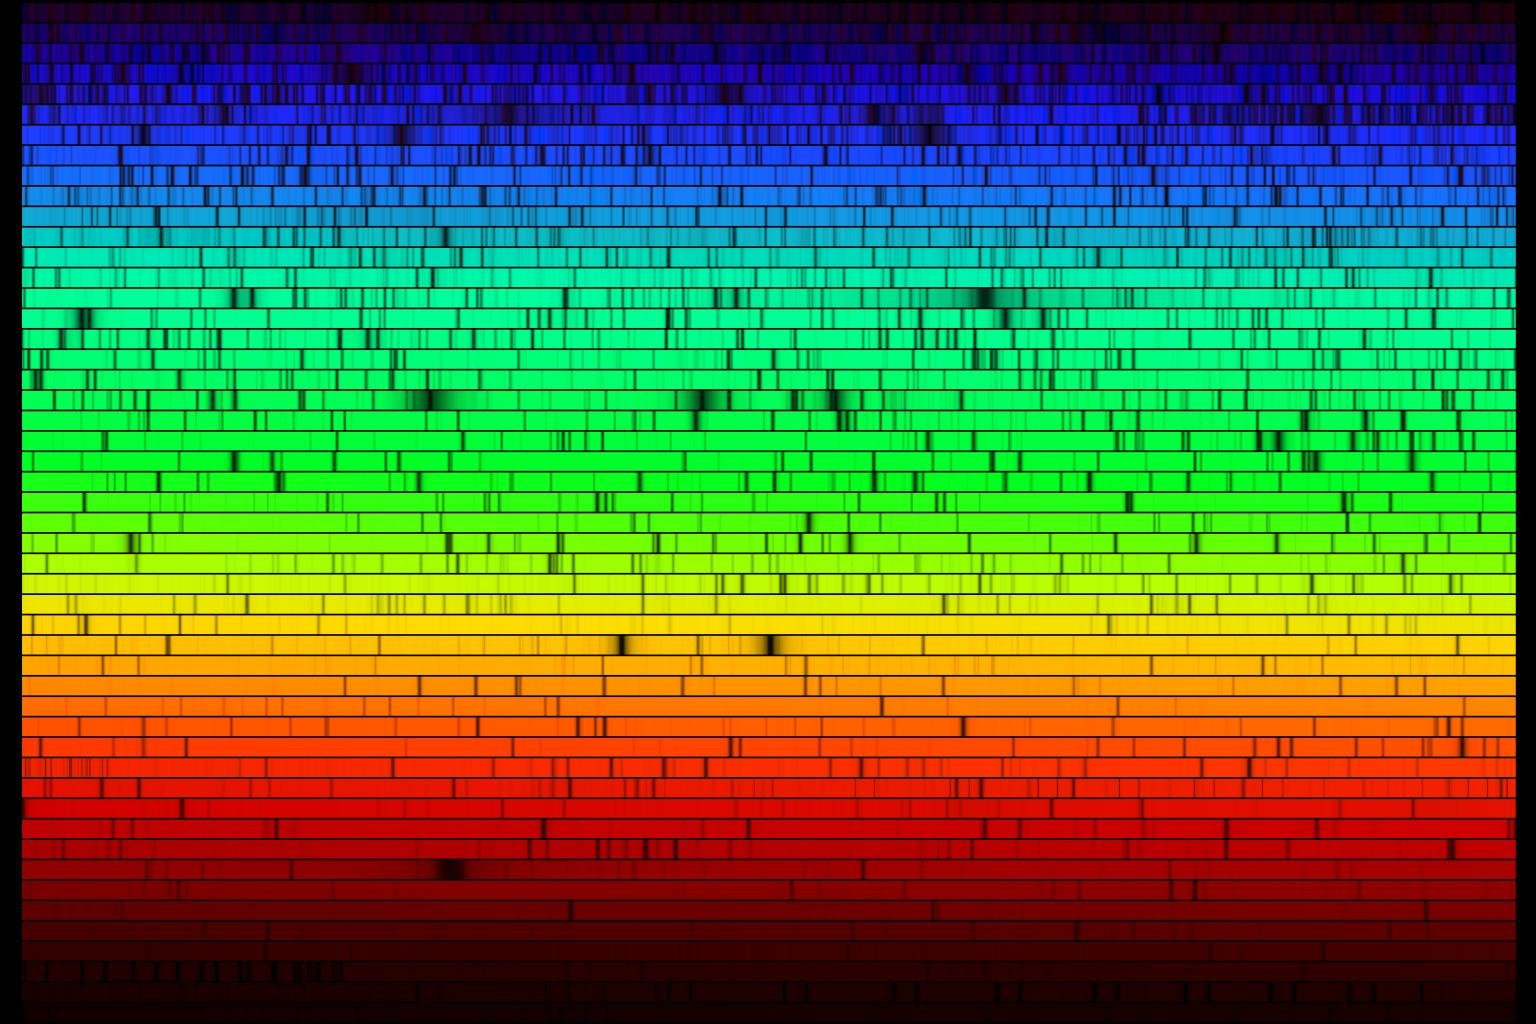
\includegraphics[width=\linewidth]{Chapter1/Figs/sun_spectrum}
	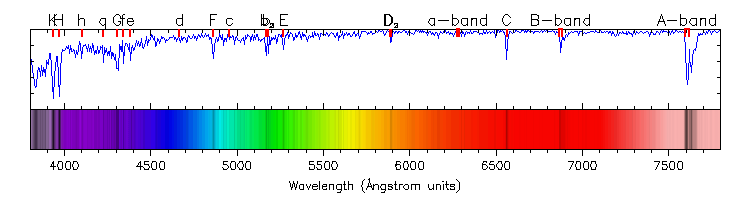
\includegraphics[width=\linewidth]{Chapter1/Figs/fraunhofer_lines}
	\caption{The top figure is a visible light measurement of the Sun. It demonstrates that there are elements in the atmosphere absorb the light and appears on this spectrum as a dark line. The Fraunhofer lines (absorption lines) are marked on a continuous spectrum with an intensity profile below.
	\url{http://media.radiosai.org/journals/Vol_05/01JAN07/04-musings.htm}}
	\label{fig:fraunhofer}
\end{figure}


Figure~\ref{fig:fraunhofer} demonstrates the white light solar spectrum, immediately apparent are the dark absorption lines.
They are a result of the quantum mechanical effects of the electron energy shells around atoms and molecules.
In the case of the Sun, a continuous spectrum is radiated from the photosphere and this light then interacts with the elements higher up in the atmosphere.
Upon collision with an atom or molecule, the exact wavelength of light which corresponds to the energy required to excite an electron from one energy level to another is absorbed by that electron.
The direct result of this is that the wavelength absorbed in the energy transaction is absent from the white-light spectrum being emitted from the photosphere, and hence appears as a dark line when observed from beyond the solar atmosphere.
These transition lines are closely aligned to the temperature at which they are formed, therefore the higher emissions lines coincide with higher temperatures.

In the case of Hydrogen, the most prevalent atom in the Sun, the array of lines generated by the transitions between energy shells is known as the Balmer series, demonstrated in Figure~\ref{fig:balmer}.
The primary line in this range is H$\alpha$, which, is widely used in solar observations as it covers the photosphere and lower chromosphere.
The complexity is that the line is broad, for example, the H$\alpha$ CRISP filter at the SST (see \ref{sec:ground}) can measure $\pm 2$ nm about the main emission line $656.28$ nm.
This allows complex analysis of solar features, but the data must be handled carefully, environmental factors such as magnetic field and temperature can alter the emission line.
\ref{ch:5} utilises the extremely detailed images provided by CRISP to calculate dopplergrams of a jet-like feature at the solar limb.

\begin{figure}
	\centering
	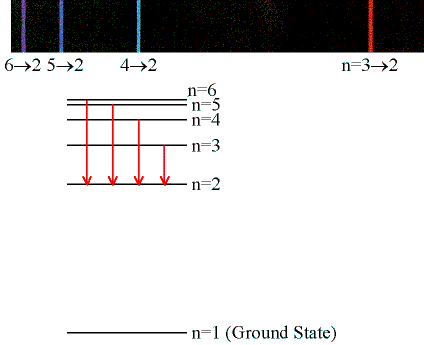
\includegraphics[scale=0.5]{Chapter1/Figs/Balmer_series}
	\caption{A demonstration of the Balmer lines, transitions in the hydrogen atoms. In this case, specifically transitions between other lines and $n = 2$.
		\url{http://www.daviddarling.info/encyclopedia/B/Balmer_series.html}}
	\label{fig:balmer}
\end{figure}

% Maybe a quick paragraph on what lines are found where.

Above the transition region iron is bounteous, and so we have many emissions lines with which to examine the corona due to the high number of available transitions.
Fe VIII ($13.1$ nm), Fe IX ($17.1$ nm), Fe XII ($19.3$ nm), Fe XIV ($21.1$ nm), Fe XVI ($33.5$ nm) and Fe XVIII ($9.4$ nm) are all observed by the spacecraft Solar Dynamic Observatory (SDO) with the Atmospheric Imaging Assembly (AIA), \cite{Schmelz2013}.
As the temperature of the atmosphere increases, the amount of available energy changes and different transitions are excited.
The various lines here therefore apply to different temperatures.

Having presented the principles with which we observe the solar atmosphere, we now need a base to image the Sun from.
% There are an array of other techniques (go into them a tiny bit)

\subsection{Observational Platforms }

In the current solar observation climate, we have a wealth of information, coming from many different sources.
Understanding the functionality of these instruments in terms of the raw method is essential to rigorous science and accurate readings.

\subsubsection{Ground-Based Telescopes}
\label{sec:ground}
Solar physics spent its early development being applied in ground-based solar telescopes, as has already been discussed, particularly in centres such as Royal Greenwich Observatory and Meudon Observatory in Paris.
In the modern era, the most powerful instruments, delivering high cadence and spatial resolution, are based on the ground..

On La Palma in the Canary Islands, at $2360$ m altitude, the Swedish Solar Telescope is situated.
The SST utilises two optical pipelines, one for the red end of the electromagnetic spectrum and another examining the blue end.
The CRisp Imaging SpectroPolarimeter (CRISP), focuses on the red end of the visible spectrum, whereas the soon to be updated instrument, Chromis, analyses the blue end.
The beam is split upon its arrival at the optical bench and sent to either of these instruments, but before the beam reaches CRISP there is a layer of correction known as adaptive optics.

As a result of the above points, the images from the SST are extremely customisable.
They are usually returned as data cubes, the dimensions of which are time, wavelength, x and y.
The resolution of these features are therefore changeable dependant on the requirements of the observation.
Cadence can be as low as $2.5$ s, the spectral increment, $0.02$ nm, and spatial resolution of $0.12$ arcsec.
Given the impressive results produced by these facilities, an ambitious new telescope is being built in Hawai'i, the Daniel K. Inouye Solar telescope (DKIST).
DKIST promises to be the most powerful solar telescope ever created with a $4$ m mirror, enabling resolution of $10$ km per pixel and overcoming the current quantity of photons issues at the limb for spectropolarimetry.



\subsubsection{Space Based Telescopes}

Space borne telescopes have a significant advantage over their ground based counterparts due to the nearly constant un-interrupted, view of the Sun without the atmospheric effects disturbing the signal.
As a result, the volume of space based instrumentation has grown exponentially since the early Skylab missions taking solar images from a low Earth orbit.

The first solar mission to move on from imagers on space stations was the Solar Heliospheric Observatory (SoHO).
Placed at the gravitationally stable Lagrange point, L1, between the Sun and Earth, it affords constant viewing of the Sun.
The mission marks a sea change in solar observations.
The range of instruments on board covered the entire solar atmosphere, [\cite{StCyr1995}], and our understanding of the Sun has been continually updated by its findings.
Originally, it was designated as a two year mission, however the mission continues to be a success and has been running for $2$ decades [\cite{Fleck2006}, \cite{Fleck2016}]
The primary scientific goals were examining photospheric behaviour, EUV imaging of the chromosphere and investigation of impactful solar weather using LASCO.

%\begin{figure}
%	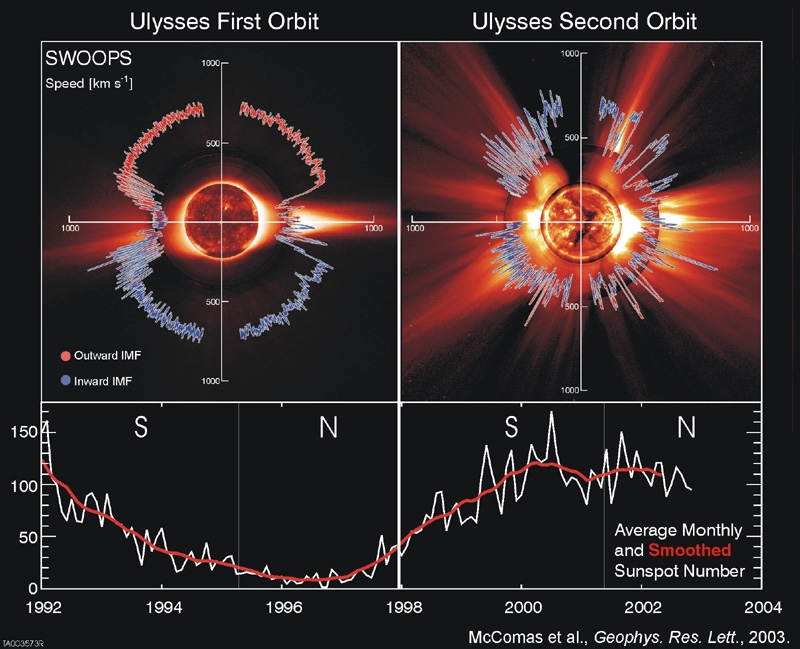
\includegraphics[scale=0.5]{Chapter1/Figs/ulysses_solar_wind}
%	\caption{The landmark solar wind measurements. On the left the solar wind during minima. A strictly divided solar wind in which high velocities are detected over the poles and lower values over the more magnetically complex equatorial quiet Sun. On the right, almost homogeneous high velocities at the solar max. This is due to a greater amount of large scale structures, such as streamers and CME's, producing fast solar wind all over the solar atmosphere.
%		\cite{McComas2003}}
%	\label{fig:ulysses_sw}
%\end{figure}


The Japanese Aerospace Exploration Agency (JAXA) have organised several solar missions.
Solar-A, renamed Yohkoh, \cite{Tsuneta1991} upon its successful launch and commencement of observations, pre-dates SoHO.
It covered soft and hard X-Ray ranges and spectrometers covering, specifically, the coronal iron lines and a wide band spectrometer. 
Yohkoh was particularly successful with respect to the detection of high energy events, and was used for Shibata's studies of X-Ray jets and their formation mechanisms.
The work undertaken my Shibata provides an excellent framework and set of 
 
JAXA's next mission was Hinode signified a significant move forward in space based solar observations, building from what was successful in Yohkoh.
The mission introduced small wavelength increment spectroscopy to space based missions.
The EUV Imaging Spectrometer (EIS) is designed to examine the chromosphere using two specific imaging techniques.
It is extremely flexible with 4 slit or slot positions, $1"$ pixel slit, $2"$ pixel slit, $40"$ pixel slot and $266"$ and two different modes for spectroscopy.

Possibly the most adventurous mission to probe the solar environment to date, is the STEREO mission (Solar TErrestrial RElations Observatory) described in \cite{Kaiser2008}.
As is suggested by the name of this mission, the primary focus was to form a more comprehensive picture of the solar atmosphere, by positioning two satellites in such an orientation to build a three dimensional picture.
Consequently, two identical satellites were launched into orbit, ahead of and behind the Earth.
There is an inherent differential in the angular velocity of the spacecraft, in order to move the spacecraft ever further around the orbit at approximately $45^\circ$ per year.
The primary objective of this stage of the mission was to obtain the optimal angle to produce three dimensional images of the Sun using a tomographic technique.

Given that STEREO was designed to give varying angles of the Sun-Earth  enviroment, the instruments on the mission are tailored to this need.
SECCHI is a suite of 5 imagers, utilising white-light coronographs, an extreme ultra violet imager and two wide angle Heliospheic Imagers (HI) designed to track CMEs to $1$ AU.
IMPACT detects solar wind electrons and the in-situ solar wind magnetic field strength and vector, while PLASTIC measures the composition of heavy ions, alpha particles and protons. 
Given the instumentation, STEREO is used extensively by space weather forecasters at NOAA, which will increasingly become an essential part of our lives.

STEREO's positioning is advantageous to this work as it affords a different viewing angle on features.
This can come in useful when considering features at the limb.
If STEREO is positioned correctly, it aid in removing uncertainty when considering possible line of sight effects.

Building on all of the above missions, the Solar Dynamic Observatory (SDO) mission began in 2010 \cite{Kaiser2008}.
The instruments are developments of concepts used on previous missions but expanding them to allow constant viewing of the entire solar disk.
Consequently all instruments on SDO view the full solar disk, at all times, maintaining the same temporal cadence. 
Therefore, the SDO mission produces significantly more raw data than any previous missions.
From a purely engineering standpoint, the instruments were carefully selected to facilitate the downloading of the data.
As such, SDO has three instruments; the Helioseismic and Magnetic Imager (HMI) examining the solar variability and finer scale structure of the solar magnetic field; the Extreme Ultraviolet Variability Experiment (EVE) measures the total solar irradiance in the Extreme Ultra Violet section of the spectrum and the Atmospheric Imaging Assembly (AIA) investigating the upper chromosphere and corona.

AIA's imaging suite provides full disk images in $4096 \times 4096$ resolution and most importantly at $12$ second cadence.
However, its distinguishing feature is the array of wavelengths analysing the atmosphere \cite{AIAspec} associated with various temperatures corresponding to the appropriate electron transitions.
The instrument ranges through $170$, $30.4$, $160$, $17.1$, $19.3$, $21.1$, $33.5$, $9.4$ and $13.1$ nm providing a temperature range of $5000$ K to $1.6 \times 10^7$ K.

Without SDO the work in this thesis would not be possible.
The constant full disk viewing greatly increases the chances of capturing the total evolution of a macrospicule.
As such, it is used extensively in all of these studies as the main observational tool in \cref{ch:3}, \cref{ch:4}, and plays an essential roll in \cref{ch:5} 


\section{Plasma behaviour}

Stars are incredibly complex features despite their apparent simplicity when viewed by the naked eye.
Their behaviour is entirely unlike any planetary body, and as has already been discussed, their inherent magnetic field makes their structure extremely complex.
All of these affects can be traced back to the fact that the Sun consists of gas kept at high temperature and pressure, which causes it to form the $4^{th}$ state of matter, plasma.
Plasma is defined as a gas in which the molecules reached an energy level that cause them to eject their outermost electrons and become ions, causing the gas to be a neutral mixture of charged ions and free electrons (produced from ionising the molecules).
It can be formed in several situations on Earth, such as a discharge of current from the atmosphere to the ground, manifesting as lightning as the propagating current ionises the air.
Plasma dynamics are significantly more complicated than those of a gas, due to the presence of inherent magnetic field. 
We therefore need a set of laws to define how the plasma behaves on scales such as those applicable on the Sun and in the atmosphere.


\subsection{Magnetohydrodynamics}

Magnetohydrodynamics are the set of laws by which we describe the motion of plasma on large scales.
They were derived by \cite{Alfven1942}, an achievement for which, Alfv{\'e}n was awarded the Nobel Prize.
The rules set up are a combination of the gas pressure equations and Maxwell's laws of electrodynamics, so let us now examine this relationship.

When considering a plasma, it is important to remember that while the total charge of the plasma will be quasi-neutral, the ions and electrons which constitute the mixture still carry charge.
Consequently, motions in the plasma will cause the charges to have a change in velocity.
In accordance with Faraday's law, a moving charge will cause a magnetic field to be induced and Ohms' law will also become a factor with charges moving through a magnetic field.
Additionally, the particles which constitute the plasma are gaseous, therefore, their motion can also be described in terms of classical fluid dynamics.
As such, this can be an extremely complex problem, let us first consider the Maxwell and gas dynamics equations.

\begin{align}
	\nabla \times \mb{E} &= -\pd{\mb{B}}{t}  &\quad \textnormal{Faradays Law}\\
	\nabla \times \mb{B} &= \mu_0\mb{j} + \frac{1}{c^2}\pd{\mb{E}}{t} &\quad \textnormal{Amp{\`e}re Law}\\
	\nabla\cdot\mb{E} &= \frac{\tau}{\epsilon_0} &\quad \textnormal{Gauss' Law}\\
	\nabla\cdot\mb{B} &= 0 & \quad \textnormal{Gauss' law of magnetism}\\
	0 &= \pd{\rho}{t} + \nabla \cdot (\rho\mb{v}) & \quad\textnormal{Equation of mass conservation}\\
	0 &= \pd{p}{t} + \mb{v}\cdot\nabla p + \gamma p\nabla\cdot\mb{v} & \quad \textnormal{Conservation of entropy}
\end{align}

\noindent where $\mb{E}$ is the electric field stength, $\mb{B}$ the magnetic field, $t$ is time, $c^2 = (\epsilon_0\mu_0)^{-1}$,$\epsilon_0$ is the vacuum permittivity, $\mu_0$ is the permeability of free space, $\mb{j}$ is the current density and $\tau$ is the charge density.
Faraday's law describes how a changing magnetic field would induce an electric field, hence it is also known as the Induction equation \citep{Goedbloed2004}.
Amp{\`e}re's law describes the manner in which the magnetic field integrated around a closed loop, related to the electric current passing through said loop.
Gauss' law for magnetism is also known as the Solenoidal condition and states that no magnetic monopoles exist and the eponymous law describes the resulting electric field caused by an electric charge.

%The common factor between these two sets of equations is the velocity vector, $\mb{v}(\mb{r},t)$, applying the equation of motion for a fluid element allows us to link them.
%The forces that would bring about such a motion would be pressure, buoyancy and Lorentz force.
%To contain the model, some assumptions will need to be made.
%First, the non-relativistic assumption, that the fluids speed will be very much less than the speed of light.
%Second, define the dimensions of $l_0$ and $t_0$ such that $v = l_0/t_0$, allowing the displacement term to be left out of the Amp{\`e}re's Law, meaning that we can neglect the effects of space charge.
%Thirdly, the non-relativistic assumption also allows the simplification to the acceleration of a fluid equation.

Combining the equations above using the velocity vector, $\mb{v}(\mb{r},t)$, and the equation of motion for a fluid element, leads to the basic equations of ideal magnetohydrodynamics (MHD):

\begin{align}
	\pd{\rho}{t} + \nabla\cdot(\rho\mb{v}) &= 0 \\
	\rho(\pd{\mb{v}}{t} + \mb{v}\cdot\nabla\mb{v}) + \nabla p - \rho\mb{g} - \frac{1}{\mu_0}(\del \times \mb{B}) \times \mb{B} &= 0\\
	\pd{p}{t} + \mb{v}\cdot\nabla p + \gamma p\nabla\cdot\mb{v} &= 0\\
	\pd{\mb{B}}{t} - \del \times (\mb{v} \times \mb{B}) &= 0\\
	\nabla\cdot\mb{B} &= 0
\end{align}

\noindent These equations are therefore applicable to the case where; 1) the plasma is strongly collisional, such that the time-scale of the collision between the particles is much smaller that the characteristic time scales of the entire system.
2) The resistivity of these collisions is small \emph{i.e.} the magnetic diffusion time scale much be longer than any other process occurring within the plasma.
3) The time-scale must be greater than that of the kinetic processes occurring within the plasma, such as ion gyration, Landau damping and length-scales longer than the ion skin depth and Larmor radius, \cite{Goedbloed2004}.

By making choices with respect to the units for length, mass and time, the MHD equations can be made dimensionless.
A typical length scale can be chosen such as $l_0$ to be something sensible and $\rho_0$ and $B_0$ are chosen from a representative point in the plasma and the time unit can be inferred from a basic speed of the plasma, \emph{e.g.} the sound speed or Alfv{\`e}n speed.

\begin{equation}
	v_0 \equiv v_{A,0} \equiv \frac{B_0}{\sqrt{\mu_0\rho_0}} \textnormal{which leads to} t_0 \equiv \frac{l_0}{v_0} 
\end{equation}

\noindent The density, velocity, magnetic field etc. are then used to define new dimensionless parameters and substituted back into the MHD equations, which remain unchanged but now a have an operator for these variables instead of the variable themselves.
The crucial outcome here is that the equations are not dependent on the size of the plasma evaluated, the magnetic field strength, the density or the time scale.
After scaling $l_0$, $B_0$ and $t_0$, the pressure term becomes of vital importance and is linked to the ratio between the kinetic pressure of the plasma and magnetic pressure.
This ratio is commonly referred to as the plasma beta, which is defined as:

\begin{equation}
	\beta \equiv \frac{2\mu_0p_0}{B_0^2}
\end{equation} 

\noindent This is and extremely useful flag when considering the behaviour of a plasma at a less precise level, as it indicates the forces dominant in a region.
If $\beta \gg 1$ the kinetic pressure terms are dominant, meaning that the kinetic motions of the plasma will determine its overall behaviour, such as in the photosphere and below.
Whereas, in the chromosphere and upwards, the balance more favours the magnetic field and the gas movement is determined by magnetic effects.
 

\subsection{Reconnection}
\label{sec:recon}

The above processes are considered to be ideal cases for energy emission, for example, the dissipation of MHD waves is an ideal solution to the problem, converting magnetic energy into kinetic energy.
The process is referred to as ideal, as it fulfils the conditions we highlighted above, that the plasma obeys Alfv{\'e}n's theorem of frozen in-flux, and that 3 premises of effects of a kinetic scale are obeyed.
However, in the reconnection process the frozen in condition is violated, as two plasma blobs which were connected by a field line, will now no longer be.
It also, impinges on the assumption that the magnetic diffusion occurs on time scales significantly greater than the dynamic phenomena within the plasma, as reconnection takes place on much shorter time scales.
This means that the reconnection mechanism itself is non-ideal.
In such processes, the magnetic energy is converted to kinetic energy and heat, more on which later.

In order for us to build a model for a reconnective event, several components are required, the magnetic field equations that describe the null point and a description of the current flowing over the change in magnetic field.
Let us begin our discussion with the null points, of which, there are two kinds, elliptical and `X-type'.
The `X-type', which can be applied to who separate magnetic field systems coming together, is the situation which occurs most regularly within the solar atmosphere so we shall consider this mechanism.

In the situation, the field lines are hyperbolic, bending away from the centre, forming an X-type neutral point, of the type applied to the solar flare problem by the authors above.
The limiting field lines are defined in terms of their angle of separation.
These lines go through the origin, and are known as separatrices, and form the characteristic 'X-type' null point. 
The $\bar{\alpha}$ value, which defines the angle between said separatrices, is related to the current density.
Which we can calculate by taking the curl of the magnetic field, \cite{Priest2007}

\begin{equation}
	\mb{j} = -\frac{B_0}{\mu_0L_0}(1 - \bar{\alpha}^2)\hat{\mb{z}}
\end{equation}

\noindent Where $\hat{\mb{z}}$ points out of the $xy$ plane.
Now we have reached the point where the current density can be discussed with respect to the null point.

The current sheet typically appears at neutral points where there is a tangential discontinuity, in which case the the magnetic field is tangential and the plasma flow across the current sheet is zero.
When the system is in equilibrium, the plasma either side of the sheet, and in the sheet itself, are in pressure balance.
Usually, the total magnetic field on the current sheet will be zero, and we assume that the ambient pressures vanish, we can say that the magnetic pressure either side of the sheet is equal to the gas pressure on it:

\begin{equation}
	\frac{B_2^2}{2\mu} = p_c = \frac{B_1^2}{2\mu}
\end{equation}

\noindent where $B_1$ and $B_2$ are the magnetic fields either side of the current sheet and $p_c$ is the gas pressure at the current sheet.
It follows that the magnetic field undergoes an exact reversal in the magnetic field.
If it is the case that the magnetic field within the sheet is parallel to the $y$ axis and varies in $x$, is defined $\mb{B} = B_y(x)\hat{\mb{y}}$, applying Amp{`e}re's law can give us the current density in $z$:

\begin{equation}
	j_z = \frac{1}{\mu}\frac{dB_y}{dx}
\end{equation}

\noindent This means that when we get a steep gradient in $B_y$ with respect to $x$, a strong current along the current sheet is produced perpendicular to the field lines.
This is the current sheet that lies at the heart of reconnection models, however the tangential discontinuity is susceptible to instabilities.
Now that we have the null point between the two magnetic fields and the current sheet that forms as a result, we have the environment necessary to begin the reconnection of magnetic field lines.

Let us consider the induction equation again defining how the magnetic field changes with respect to the magnetic field,

\begin{equation}
	\pd{\mb{B}}{t} = \del \times (\mb{v} \times \mb{B}) + \eta\del^2\mb{B}
\end{equation} 

\noindent with the first term representing the advection and the second the diffusivity of the magnetic field.
The ratio of these two terms can be represented by the magnetic Reynolds number, $\Re_m = LV/\lambda$, and of course, this value will dictate the evolution of the induction.
The diffusion term dominates in the case where $\Re_m \ll 1$, however, we must be aware that this condition will not apply on large scales in the solar atmosphere, although it may be true on very small scales.
The second mechanism for the changing of the magnetic field lines is advection. 
Under the condition $\Re_m \gg 1$, we drop the diffusive term from the induction equation.






